% ------------------------------------------------------------------------------
% layout
\documentclass [twoside]{scrreprt}                % [] 10pt|11pt|12pt font size, default 10pt
	  \KOMAoptions{paper=a4}

% encoding stuff
\usepackage [utf8]{inputenc}
\usepackage [T1]{fontenc}                         % fuer korrekte trennung deutscher umlaute, scharf-s etc.


% figures
\usepackage {pgf}                                 % includepgf for bitmaps
\usepackage {epsfig}
\usepackage {psfrag}                              % replacing strings in eps files
%\usepackage [bf,small]{caption}                   % caption style
\usepackage {ifpdf}
%\ifpdf
    \usepackage{graphicx}
    \usepackage{epstopdf}
    %\DeclareGraphicsRule{.eps}{pdf}{.pdf}{`epstopdf #1}
    \pdfcompresslevel=9
%\else
  %  \usepackage {graphicx}
%\fi

\usepackage {subfig}                              % subfigures a) b)...
%\usepackage {floatflt}                           % packages supporting in-text floats
%\usepackage {wrapfig}                            % another one
%\usepackage {picins}                             % another one
%\usepackage{timing}                              % deprecated use, use below!
\usepackage{tikz-timing}                          % timing diagrams
\usepackage{sidecap}

\usepackage{listings}
\lstset{
    frameround=fttt,
    language=C,
    %numbers=left,
    breaklines=true,
    keywordstyle=\color{red}\bfseries, 
    basicstyle=\ttfamily,
    numberstyle=\color{black}
    }
\lstMakeShortInline[columns=fixed]|


% tables
\usepackage{multirow}                             % col- and rowspan...
\usepackage{booktabs}                             % professional table layout


% math
\usepackage{bbm}                                  % black board style, (e.g. \mathbbm{R})
\usepackage{amssymb}
\usepackage{amsmath}                              % e.g. \nobreakslash- for non-breakable hyphens
\usepackage{bbold}
\usepackage{amsfonts}
\usepackage{units}

% text
\usepackage {latexsym}                            % additional symbols
%\usepackage{lmodern}                              % latin modern
\usepackage [english,ngerman]{babel}              % language (change via "\selectlanguage{english}")
%\usepackage[colorlinks=true,pdftex=true,linkcolor=black,citecolor=black,urlcolor=blue,plainpages=false,pdfpagelabels]{hyperref}
\usepackage[colorlinks=true,linkcolor=black,citecolor=black,filecolor=black,urlcolor=black,plainpages=false,pdfpagelabels,breaklinks=true]{hyperref}
%\usepackage[all]{hypcap}                          % links to figures point to upper border (not caption)
\usepackage{breakurl}
\usepackage{hyphenat}
\usepackage[normalem]{ulem}                       % underline text...
\usepackage{listings}                            % source/code listings
\usepackage[plain]{algorithm}
\usepackage{algorithmicx}                        % pseudo code
\usepackage{algpseudocode}                       % pseudo code
\usepackage{units}                               % \unit[123]{U}
\usepackage{mdwlist}                             % dichtere itemize* etc.
\usepackage{paralist}                            % inline Listen
\usepackage{natbib}


% list of abbreviations, index
\usepackage{nomencl}
    \let\abbrev\nomenclature
    \renewcommand{\nomname}{List of Abbreviations}
    \setlength{\nomlabelwidth}{.25\hsize}
    \renewcommand{\nomlabel}[1]{#1 \dotfill}
    \setlength{\nomitemsep}{-\parsep}
    %\makeglossary
    \makenomenclature
    \newcommand{\markup}[1]{\uline{#1}}
\usepackage{makeidx}                              % index of key words
    \makeindex


% layout
\usepackage{todonotes}
%\usepackage{stfloats}
%\usepackage{dblfloatfix}
\usepackage{fixltx2e}
%\usepackage {afterpage}                          % \afterpage{xyz} executes xyz after current page is finished
%\usepackage {flafter}                            % no object before definition
%\usepackage {float}                              % Here(!!!) placement option
% ------------------------------------------------------------------------------


% source aliases
\newcommand{\thesisTitle}{Bachelor Thesis}
\newcommand{\thesisTitleGerman}{German Title}
\newcommand{\thesisAuthor}{Arthur Heimbrecht}
\newcommand{\thesisAuthorBornIn}{Speyer}



% hypenation (englisch)
\selectlanguage{english}
\hyphenation    {HAGEN HASTE HANNEE Bert-schin-ger Maass ma-xi-mum SoftHASTE
neu-ron pre-synaptic post-synaptic}

% hypenation (deutsch)
\selectlanguage{ngerman}
\hyphenation    {HAGEN HASTE HANNEE Bert-schin-ger Maass SoftHASTE}


\tolerance 1414
\hbadness 1414
\emergencystretch 1.5em % critical parameter!!!
%\displaywidowpenalty % avoid widows after math displays
\raggedbottom % should be default anyway
%\clubpenalty = 10000
%\widowpenalty = 10000
%\hfuzz 0.3pt
%\vfuzz


%\renewcommand{\bottomfraction} {0.70} % max fraction of page for floats at bottom
%\renewcommand{\textfraction} {0.20} % min fraction of page for text
%\renewcommand{\floatpagefraction} {0.60} % min fraction of floatpage that should have floats
%\renewcommand{\dblfloatpagefraction}{0.60} % for twocolumn layout, see floatpagefraction above
%\setcounter{totalnumber} {6} % max number of floats on a single page
%\setcounter{topnumber} {6} % max number of top floats on a single page
%\setcounter{dbltopnumber}{6} % for twocolumn layout, see topnumber above
%\setcounter{bottomnumber}{6} % max number of bottom floats on a single page
% ------------------------------------------------------------------------------

\pagestyle  {empty}                               % plain, empty, headings oder myheadings.



\begin{document}

% ------------- Cover Pages ----------------------

\begin{titlepage}

\textwidth 		14cm
\textheight 		27.0cm

\evensidemargin    	-1.5cm
\oddsidemargin   	-1.5cm
\topmargin     		-3.0cm

\thispagestyle{empty}


\begin{figure}

\includegraphics{fig/cover/Publ-Cover1.eps}
%\epsfig{file=./fig/cover/Publ_Cover1.eps}% , width=\textwidth}%,height=4.5cm}
\end{figure}

\vspace*{3cm}

\hspace{5cm}
\begin{minipage}{8.2cm}
\begin{flushright}
\Large{\sf{\thesisAuthor}}
\end{flushright}
\end{minipage}


\begin{figure}[ h]

\includegraphics{fig/cover/Publ-Cover2.eps}
%\epsfig{file=./fig/cover/Publ_Cover2.eps}%,width=12.7cm}
\end{figure}

\vspace*{3mm}

\hspace{3cm}
\begin{minipage}{10.2cm}
\begin{flushright}
\Large{\sf{\thesisTitle}}
\end{flushright}

\vspace*{3mm}

\vspace*{4mm}

\begin{flushright} \Large{\sf{
%%% no = fortlaufende KIP-Nummer, wird von der Bibliothek (Tel. 8992) vergeben.
%HD-KIP-04-16
}}
\end{flushright}

\end{minipage}


\begin{figure} [b]

\includegraphics{fig/cover/Publ-Cover3.eps}
%\epsfig{file=./fig/cover/Publ_Cover3.eps}%,width=12.7cm}
\end{figure}

\end{titlepage}


\cleardoublepage
\begin{titlepage}

\begin{center}
\vspace*{2cm}
\huge{\bf{Department of Physics and Astronomy}} \\
\vspace*{0.2cm}
\LARGE{\bf{University of Heidelberg}}
\end{center}
\vspace*{10cm}
%\vfill
\large
\begin{center}
{\bf{Bachelor Thesis}} \\
\vspace*{0.2cm}
in Physics\\
\vspace*{0.2cm}
submitted by\\
\vspace*{0.2cm}
\textbf{\thesisAuthor}\\
\vspace*{0.2cm}
born in \thesisAuthorBornIn\\
\vspace*{1cm}
\textbf{TODO 2123}
\end{center}

\end{titlepage}


%\begin{titlepage}

\begin{center}
\vspace*{2cm}
\huge{\bf{Fakultät für Physik und Astronomie}} \\
\vspace*{0.2cm}
\LARGE{\bf{Ruprecht-Karls-Universität Heidelberg}}
\end{center}
\vspace*{10cm}
%\vfill
\large
\begin{center}
{\bf{Bachelorarbeit}} \\
\vspace*{0.2cm}
im Studiengang Physik\\
\vspace*{0.2cm}
vorgelegt von\\
\vspace*{0.2cm}
\textbf{\thesisAuthor}\\
\vspace*{0.2cm}
geboren in \thesisAuthorBornIn\\
\vspace*{1cm}
\textbf{TODO 2123}
\end{center}

\end{titlepage}



\cleardoublepage
\begin{titlepage}

\begin{center}
\vspace*{2cm}
\huge{\textbf{\thesisTitle}}\\
%\huge{\bf}\\
\end{center}
\vspace*{10cm}
%\vfill
\large
\begin{center}
{\bf This Bachelor Thesis has been carried out by \thesisAuthor{} at the} \\
\vspace*{0.2cm}
{\sc Kirchhoff Institute for Physics\\

\vspace*{0.2cm}
Ruprecht-Karls-Universität Heidelberg\\}
\vspace*{0.2cm}
{\bf under the supervision of}\\
\vspace*{0.2cm}
{\bf Prof. Dr. Karlheinz Meier}\\
\end{center}

\clearpage

\vspace*{15cm}
\begin{center}
%For someone.
\end{center}


\end{titlepage}


%\begin{titlepage}

\begin{center}
\vspace*{2cm}
\huge{\textbf{\thesisTitleGerman}}\\
%\huge{\bf}\\
\end{center}
\vspace*{10cm}
%\vfill
\large
\begin{center}
{\bf Diese Bachelorarbeit wurde von \thesisAuthor{} ausgeführt am} \\
\vspace*{0.2cm}
{\sc Kirchhoff-Institut für Physik\\

\vspace*{0.2cm}
Ruprecht-Karls-Universität Heidelberg\\}
\vspace*{0.2cm}
{\bf unter der Betreuung von}\\
\vspace*{0.2cm}
{\bf Prof. Dr. Karlheinz Meier}\\
\end{center}

\clearpage

\vspace*{15cm}
\begin{center}
%For someone.
\end{center}


\end{titlepage}



%-------------------------------------------------






% and now in englisch!
\selectlanguage{english}





% ------------- Abstract -------------------------

\cleardoublepage

\pagestyle{plain}

\setcounter{page}{1}
\pagenumbering{Roman}

\begin{abstract}
\begin{center}
\textbf{\thesisTitle}
\end{center}

As part of the Human Brain Project, BrainScaleS is a unique project on many levels. This includes a processor solely used by the HICANN-DLS, which manages synaptic weights for every neuron built into one of the many wafers. To accelerate the speed at which this so called plasticity processor unit (PPU) computes all synaptic weights of every neuron used, the processor has an extended instruction set architecture (ISA) that supports vector registers and single input multiple data (SIMD).
This report deals with the task of adding built-in functions to an existing back-end of GCC, specifically the one used by the PPU, in order to extend the already implemented set of functions according to the users needs.
\end{abstract}


%-------------------------------------------------




% ------------- Table of Contents ----------------

\cleardoublepage
\setcounter{tocdepth}{3}
\tableofcontents

%-------------------------------------------------






% ------------- Chapters -------------------------

\cleardoublepage

\pagestyle{headings}

\setcounter{page}{1}
\pagenumbering{arabic}



%%% INCLUDES %%%%%%%%%%%%%%%%%%%%%%%%%%
% introduction
\chapter{Introduction}
\label{chapter:introduction}

Neuromorphic computing has developed into a popular scientific field throughout the last years and finds more and more applications and implementations in science and industry, e.g.~\cite{6905473}.
These systems already show advantages over traditional computer architectures, like the von-Neumann architecture, in specific applications and continue to improve.
In its current generation, neural networks abandon discrete time steps and states, but gain more computational power~\cite{Maass19971659}.
They use spikes and continuous time scales that resemble nature more closely and allow for efficient implementations as analog hardware which offers high performance at low energy consumption~\cite{NIPS2015_5862}.
Still, new architectures also require novel styles of programming~\cite{Amir2013CognitiveCP} and users need to adapt to these.
This can be a hurdle for many users when developing new experiments, that initially take a significant amount of time. 
\\
\\
One example for this is the current way of programming for the plasticity processing unit of the \ac{HICANN-DLS}. 
The \ac{HICANN-DLS} is a small scale system that features analog emulation of neurons and synapses in networks~\cite{PPU}.
The \ac{PPU}, as part of \ac{HICANN-DLS}, can be used for implementing plasticity rules for such networks.
It resembles a traditional processor architecture, which was modified for this task.
Implementing such plasticity rules differs from conventional high-level programming styles. 
When creating code for the \ac{PPU}, users are partially pushed back to the origins of computing;
instead of assigning values like |d = a + b|, one must first read the variables from memory, then operate on their values and finally write back the result to memory.
Therefore coding for the \ac{PPU} works on a low level and brings new challenges to users, that are already challenged by neuromorphic programming.

Ultimately, the more a system abandons conventional elements of programming, the more challenges emerge from this.
Although experienced programmers can create highly efficient code like this, normal users will not be familiar with this.
This can cause fewer users to take the initiative of writing code for such systems, but also can code get confusing, hard to debug and even inefficient.
\\
\\
Compilers usually save users from these problems by offering high-level languages.
Over decades compilers have been developed and became a standard tool for programmers.
At the same time compilers became more and more of a black box that transforms a program into an executable file.
For this reason it may be difficult for some users to abandon their convenience and go back to low-level programming.

Though the \ac{PPU} is not completely without compiler support, its distinct features are only usable on a low level.
As these features are necessary to implement plasticity rules on the \ac{HICANN-DLS}, this can easily cause inconveniences for users.
Users repeatedly have to mix high-level and low-level code, which is an atypical style of programming.
It can cause different problems, as users have to adapt to this and, in the beginning, likely create bugged or inefficient programs.
As performance is important for neuromorphic programming, users may need an unreasonable amount of time and work to achieve simple results with this.
\\
\begin{wrapfigure}{R}{0.5\textwidth}
\captionsetup{format=plain, indention=.6cm, labelsep=newline,singlelinecheck=false}
    \centering
    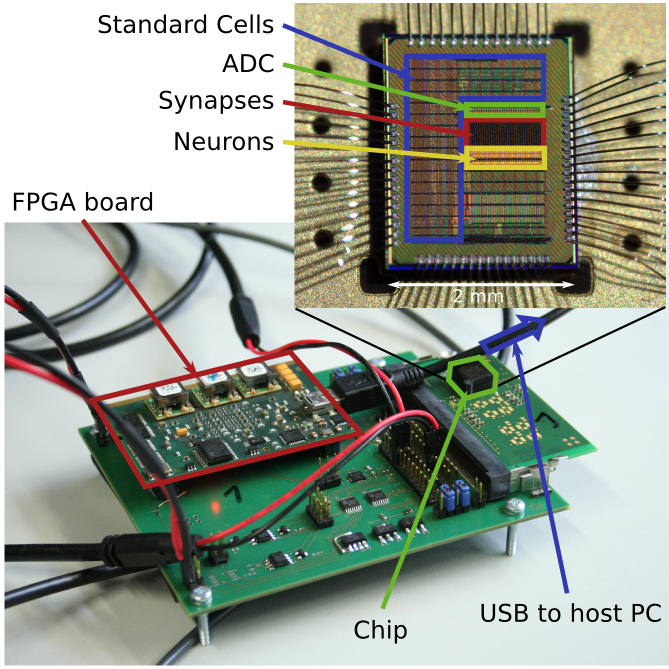
\includegraphics[width=0.4\textwidth]{pictures/Fig1.png}
    \caption{\label{fig:dlsboard} Set-Up of a \ac{HICANN-DLS} Test System (from~\citeauthor{PPU})}
\end{wrapfigure}
\\
Until now full compiler support does not exist for the \ac{PPU} because of its modified processor architecture, which was developed solely for neuromorphic hardware.
It offers a partly customized instruction set that is optimized for its applications.
\\
The \ac{HICANN-DLS} already is an experimental platform, which is used by several users, even though of \ac{PPU}-related challenges.
Applications like in-the-loop training or \ac{STDP} have been developed and mostly do not involve the \ac{PPU} .
Even when taking the effort of learning to code for the \ac{PPU}, users are constantly challenged by missing programming features such as creating parameterized functions.
This leads to repetitive code or difficulties when integrating calibration into experiment-related code.

Offering more tools for \ac{PPU} programs could reduce the effort of developing for the \ac{PPU}, while at the same time increasing capabilities of programs.
Besides allowing full high-level programming, compiler support could also offer tools like code optimization and debugging features.
At some point compiler support may also facilitate automatic code generation as a prerequisite for implementation of very high-level languages.
Users then could create plasticity rules in existing program environments from where code is translated into \ac{PPU} programs.
This creates the need for optimization of \ac{PPU} code, like those built into virtually every compiler.
\\
\\
This thesis will focus on achieving aforementioned compiler support and briefly explain the process itself.
As fundamental knowledge of both, processors and compilers, is needed along the way, the second chapter will start with a very basic introduction to both topics.
This involves basic information about the \ac{PPU}, as well as the \ac{GCC}, and should explain the basic concepts to an extend which is sufficient.
Afterwards, the process of extending the compiler is explained, followed by a presentation of results as well as first test cases.
The thesis will conclude in a resume and give an outlook to future applications and development of the compiler and the \ac{PPU}.


\chapter{Neural Networks and Implementation in Hicann-DLS}
\label{chapter:networks}

This thesis mainly focuses on an essential part of the HICANN-DLS system.
HICANN-DLS stands for \todo{what does hicann stand for?} Digital Learning System.
For this reason it is important to understand the basics behind this and what the PPU is meant to do.

\section{Basics of Neural Networks}
Neural networks build the main application of the Hicann DLS system. This short chapter is meant to give an overview over neural networks and synaptic weights.

On a very abstract level neurons in the brain resemble nodes of a network.
As in a network neurons are interconnected through dendrites, synapses and axons which can be of different strength. 
Also we assume that a neuron is either spiking, meaning it is activated and sends this information to connected neurons or resting meaning it is not activated.
In case a neuron is spiking, it send this information through its axon to other other neurons that are connected to the axon by synapses.
These synapses can work quite differently but have in common that there is a certain weight associated to them, which we will call synaptic weight.
This is equal to a gain with which the signal is either amplified or damped \todo{ is this word right?}.
The signal is then passed through the dendrite of the post-synaptic neuron to the soma where all incoming signals are integrated.
If the integrated signals reach a certain threshold the neuron spikes and then sends a signal itself to other neurons.

With all these physiological parts there are only two important parts we need to take a look at in order to copy the function of a neural network: the neuron and the synapses.
Basically we assume that all neurons are connected to each other through some synaptic weight.
If two neurons are actually not meant to be connected, the synaptic weight simply is set to zero for these neurons to be disconnected.
Now if we display the all neurons inputs and outputs in a 2D plain we get an array of synapses, which is equivalent to a weight matrix.

\section{Implementation in Hicann-DLS}
The Hicann-DLS system tries to implement this structure as close to reality as possible in order to simulate physiological processes in such networks.
At its core it therefore has a so called ``synaptic array" that connects 32 neurons which are located on a single ship to 64 different inputs.
Each neuron's input is aligned along one axis of an array while the 64 outputs of different neurons are on a rectangular axis.
This gives a 2D array of 2048 synapses in total.
The FPGA connects the 64 outputs of the synapse array to neurons in the system while it can also connect the neurons on the same chip to the output channels.
Along each output channel the signal reaches all synapses where it is proccsed.
Each synapse then multiplies the signal it receives with its own weight and sends the result to the inputline of a neuron.
All signals sent by synapses to an input are integrated along the line to a resulting input signal which finally reaches a neuron.
This is not done continuously but discretely and the output signals of all neurons are sent out at the same time.
The output signal of each neuron is also sent to an analogue digital converter (ADC) in order to analyze the data in digital form.
Inside the neurons the individual input signal is evaluated in regard to a threshold and other parameters which decide whether the neuron is spiking or not.
If the neuron is spiking it sends out an output signal to the FPGA which is responsible for spike routing.

The Hicann-DLS system is also equipped with a processing unit that includes a vector extension and some memory for it to operate on.
This is the plasticity processing unit (PPU) which is also connected to the synapse array and thus can read and write synaptic weights.

The whole chip itself is also connected to a field programmable gate array (FPGA) that is able to read and write to the synaptic values as well as the memory of the PPU.
In general the PPU is meant to simulate plasticity of the synapses during experiments while the FPGA should be used to initially set up an experiment and record data.
Therefore the PPU can also read out spiking rates and other additional information of neurons as they are needed for plasticity.
This is realized through the same omnibus that connects the PPU to the memory and virtually the spiking times are accessible through a pointer with a special address.

The synapses in the synapse array are realized as small repetitive circuits that contain 8 bits of information each.
The first two of these bits are used for calibration while the other 6 

\subsection{The plasticy processing unit}

\add{
CURRENT STATE OF PROGRAMMING ON HICANN -> MOTIVATION
main feature analogue spiking
PPU can read spiking times
size and alignment of weights 
read paper first
64 outputs
32 inputs to 32 neurons

}


\chapter{The HICANN DLS system}
\label{chapter:hicann}

This thesis mainly focuses on an essential part of the HICANN-DLS system.
HICANN-DLS stands for \todo{what does hicann stand for?} Digital Learning System.
For this reason it is important to understand the basics behind this and what the PPU is meant to do.

First of all 



\tcbset
{enhanced,colframe=blue!70!black,colback=white!50!blue,colupper=red!50!black,
fonttitle=\bfseries,center title, size=small}

\centering

%\begin{tcolorbox}[enhanced jigsaw, width=\linewidth, remember as=pp, opacityframe=0.0, opacityback=0.0, nobeforeafter]
\tcbset
{enhanced,colframe=blue!70!black,colback=white!50!blue,colupper=red!50!black,
fonttitle=\bfseries,nobeforeafter,center title, noparskip, size=small}

\begin{tikzpicture}[line width=1mm]
    
    \node[] (c) at (0,0) {
    \begin{tcolorbox}[width=.65\linewidth, enhanced jigsaw, remember as=cpu, size=normal]
        \centering
        Processor
    
        \begin{tcolorbox}[enhanced jigsaw, noparskip,opacityframe=0.3, opacityback=0.3, width=\linewidth, height=.7cm, size=small, remember as=cs]
        \centering
        Control Section
        \end{tcolorbox}
    
        \begin{tcolorbox}[enhanced jigsaw, noparskip,opacityframe=0.3, opacityback=0.3, width=\linewidth, size=small, fontupper=\footnotesize]
            \centering
    
            \begin{tcolorbox}[enhanced, width=\linewidth, remember as=alu]
                \centering
                ALU
            \end{tcolorbox}
            \begin{tcolorbox}[enhanced, width=\linewidth, remember as=rf]
                \centering
                Register File
            \end{tcolorbox}
    
            Operational Section
        \end{tcolorbox}
    
    \end{tcolorbox}
    };
    \end{tikzpicture}
    
\begin{tikzpicture}[overlay,remember picture,line width=0.5mm]
    
    \node[] (a) at ($(cs.west)!.0!(cs.north west)-(1.5,0)$) {
        \begin{tcolorbox}[enhanced jigsaw, opacityframe=0.3, opacityback=0.3, height=0.7cm, width=.15\linewidth, remember as=in, watermark text=Input, nobeforeafter]
        \end{tcolorbox}
    };
    
    \node[] (b) at ($(cs.east)!.0!(cs.north east)+(1.5,0)$) {
    \begin{tcolorbox}[enhanced jigsaw, opacityframe=0.3, opacityback=0.3, height=0.7cm, width=.15\linewidth, remember as=out, watermark text=Output, nobeforeafter]
    \end{tcolorbox}
    };
    
    \draw[->, shorten >=-1.0mm] (in.east) -- ($(cs.west)!.0!(cs.north west)$);
    \draw[->, shorten >=-1.0mm] ($(cs.east)!.0!(cs.north east)$) -- (out.west);

    \draw[->, shorten >=-1.0mm] ($(cs.west)!.5!(cs.south west)$) to [out=225, in=180] (alu.west);
    \draw[->, shorten >=-1.0mm] (alu.east) to [out=20, in=315] ($(cs.east)!.5!(cs.south east)$);
    
    \draw[->, shorten >=-1.0mm] ($(alu.south)!.5!(alu.south east)$) -- ($(rf.north)!.5!(rf.north east)$);
    \draw[->, shorten >=-1.0mm] ($(rf.north)!.5!(rf.north west)$) -- ($(alu.south)!.5!(alu.south west)$);
\end{tikzpicture}


% \begin{tikzpicture}[overlay,remember picture,line width=1mm]
%     \draw[->, shorten >=-1.5mm] ($(cp.north)+(0,1)$) -- (sc.north);
%     \draw[->, shorten >=-1.5mm] (sc.south) -- (ps.north);
%     \draw[->, shorten >=-1.5mm] (ps.south) -- (sa.north);
%     \draw[->, shorten >=-1.5mm] (sa.south) -- (sco.north);
%     \draw[-] (sco.south) -- (me.north);
%     \draw[->, shorten >=-1.5mm] (me.south) -- (cg.north);
%     \draw[->, shorten >=-1.5mm] (cg.south) -- (tco.north);
%     \draw[->] (tco.south) -- ($(cp.south)+(0,-1)$);
% \end{tikzpicture}
% \begin{tikzpicture}[overlay,remember picture,line width=1mm]
%     \draw[-, draw=blue!30!white,line width=.5mm, shorten >=.2cm,shorten <=.1cm] (cmp.north east) -- (cp.north west);
%     \draw[-, draw=blue!30!white,line width=.5mm, shorten >=.2cm,shorten <=.1cm] (cmp.south east) -- (cp.south west);
% \end{tikzpicture}

% chapter 1

    \tcbset
    {enhanced,colframe=blue!70!black,colback=white!50!blue,colupper=red!50!black,
    fonttitle=\bfseries,nobeforeafter,center title, noparskip}
    \noindent{\begin{minipage}{\textwidth}
        \begin{minipage}[c][][c]{0.25\textwidth}
            \begin{tcolorbox}[tcbox raise base, width=\linewidth, remember as=cp, enhanced, watermark text=Compiler]
                \begin{tcolorbox}[enhanced, breakable, noparskip,opacityframe=0.0, opacityback=0.0, height=2cm, width=\linewidth]
                \end{tcolorbox}
                \begin{tcolorbox}[enhanced, breakable, noparskip,opacityframe=0.0, opacityback=0.0, height=1cm, width=\linewidth]
                \end{tcolorbox}
                \begin{tcolorbox}[enhanced, breakable, noparskip,opacityframe=0.0, opacityback=0.0, height=1.5cm, width=\linewidth]
                \end{tcolorbox}
            \end{tcolorbox}
            \begin{tikzpicture}[overlay,remember picture,line width=1mm]
                \draw[->, shorten >=-1.5mm] ($(cp.north)+(0,1)$) -- node [left] {program code} (cp.north);
                \draw[->] (cp.south) -- node [left] {machine files} ($(cp.south)+(0,-1)$);
            \end{tikzpicture}
        \end{minipage}
\end{minipage}}


% chapter 2
\chapter{Insn-Coding}
\label{chapter:insn coding}

The PPU, which was designed by Simon Friedmann \todo{PPU paper}, is a custom processor, that is based on the Power Instruction Set Architecture (PowerISA), which was developed by IBM since 1990. The specifically the PPU uses POWER7 which is a successor of the original POWER architecture and was released in 2010.

The PPU's distinct feature is its vector unit or vector extension that allows for Single Input Multiple Data (SIMD) operations.
This was added due to the need for fast handling and writing of the synaptic weights into the array of synaptic values on the HICANN.
Specifically the vector extension allows for either use of 8 element vectors with element being halfword (1 halfword = 2 bytes) sized or 16 element vectors with each element byte sized
Thus every vector is 16 bytes or 128 Bits long.
This is also the size of each vector register that is available, 32 in total, in contrast to 32 general purpose registers with 32 bit each.
Also there is an accumulator featured as part of the vector extension which is used in every arithmetic operation and a condition register which holds 3 bits, that determine which condition applies, for every half byte or nibble, making 96 bit in total.
\todo{add special regs of normal prcessro part, CC, LR, etc.}
The PPU also features 4 KiB of memory as well as access to the synapse array of the HICANN which holds up to 32x32, thus 1024 different values.
To handle the vector unit the instruction set was extended by xz \todo{count number of vector istructions.} new instructions that partly share their opcodes with existing AltiVec instructions.

\todo{theoretical gain in speed when using vector unit compared to normal instructions especially with single load and store. include PPU clock frequencies for each part in calculation.}

% chapter Y
%\input{tex/Y}

% discussion
\chapter{Discussion}
\label{chapter:discussion}

Discussion...


% outlook
\chapter{Outlook}
\label{chapter:outlook}

As it was hinted in the discussion of this report, there are plans on extending the rs/6000 back-end of GCC so it supports the PPU's vector unit
This is surrently in the works currently as there are even some PPU-specific intrinsics already. Because the PPU is a simple PowerISA chip with a custom vector unit the implementation of intrinsics is easily transferable from the AltiVec vector extension to the PPU by swapping the |ALTIVEC| keyword with |S2PP|. With some knowledge of RTL this report then allows to add new composite intrinsic functions based on the instruction set of the PPU. By then this guide should be accompanied by a more complex thesis that explains the extension of the rs/6000 back-end and is meant to provide the reader with more insight into things like RTL and maybe makes reading the GCC internal obsolete.

%%%%%%%%%%%%%%%%%%%%%%%%%%%%%%%%%%%%%%%%





\appendix

\addcontentsline{toc}{chapter}{Appendix}
\chapter*{Appendix}

\section*{Acronyms}
\begin{acronym}
    \acro{ADC}{Analogue Digital Converter}
    \acro{ALU}{Arithmetic Logic Unit}
    \acro{ASIP}{Application Specific Instruction set Processor}
    \acro{asm}{Assembly}
    \acro{CADC}{Correlation Analogue Digital Converter}
    \acro{CISC}{Complex Instruction Set Computer}
    \acro{CPU}{Central Processing Unit}
    \acro{CR}{Conditional Register}
    \acro{DLS}{Digital Learning System}
    \acro{DRAM}{Dynamic RAM}
    \acro{insn}{instruction}
    \acro{IR}{Intermediate Representation}
    \acro{FPGA}{Field Programmable Gate Array}
    \acro{FPR}{Floating Point Register}
    \acro{FPU}{Ploating Point Unit}
    \acro{GCC}{GNU Compiler Collection}
    \acro{GPP}{General Purpose Processor}
    \acro{GPR}{General Purpose Register}
    \acro{HICANN}{High Input Count Neural Network}
    \acro{HICANN-DLS}{High Input Count Neural Network - Digital Learning System}
    \acro{ISA}{Instruction Set Architecture}
    \acro{LLVM}{Low Level Virtual Machine}
    \acro{LR}{Linker Register}
    \acro{LRA}{Local Register Allocator}
    \acro{MMU}{Memory Management Unit}
    \acro{MSB}{Most Significant Bit}
    \acro{nux}{alternative name for PPU}
    \acro{POWER}{Performance Optimization With Enhanced RISC}
    \acro{PPU}{Plasiticty Processing Unit}
    \acro{RAM}{Random Access Memory}
    \acro{RF}{Register File}
    \acro{RTL}{Register Transfer Language}
    \acro{RISC}{Reduced Instruction Set Computer}
    \acro{rs6000}{RISC system/6000}
    \acro{s2pp}{synaptic plasiticity processor}
    \acro{SIMD}{Single Input Multiple Data}
    \acro{SPR}{Special Purpose Register}
    \acro{SRAM}{Static RAM}
    \acro{VE}{Vector Extension}
    \acro{VR}{Vector Register}
    \acro{VSCR}{Vector Status and Control Register}
    \acro{VRSAVE}{Vector Save/Restore register}
    \acro{VRF}{Vector Register File}
    \acro{VMX}{Vector Media eXtension}

\end{acronym}

\section*{List of nux Intrinsics}

\begin{table}
    \adjustbox{max width=\textwidth}{%
        \begin{tabular}{c c¡c¡c¡c¡c¡p{5cm}}
            \multicolumn{1}{c}{intrinsic name} & \multicolumn{1}{c}{use} & \multicolumn{4}{c}{data types} & \multicolumn{1}{c}{effect}\\
            \cline{3-6}
             & & d & a & b & c & \\
            \hline \hline
                \begin{tabular}[x]{@{}c@{}}|fxv_add|\\|vec_add|\end{tabular} & |d = fxv_add(a,b)| & same as |a| & 
                \begin{tabular}[x]{@{}c@{}} |vector signed char|\\
                                            |vector unsigned char|\\
                                            |vector signed short|\\
                                            |vector unsigned short|\end{tabular}
                                            & same as |a| & &  add |a| and |b| modulo element-wise and write the result in |d|\\ 
            \cline{3-6}
                \begin{tabular}[x]{@{}c@{}}|fxv_sub|\\|vec_sub|\end{tabular} & |d = fxv_sub(a,b)| & same as |a| & 
                \begin{tabular}[x]{@{}c@{}} |vector signed char|\\
                                            |vector unsigned char|\\
                                            |vector signed short|\\
                                            |vector unsigned short|\end{tabular}
                                            & same as |a| & &  subtract |b| from |a| modulo element-wise and write the result in |d|\\ 
            \cline{3-6}
                \begin{tabular}[x]{@{}c@{}}|fxv_mul|\\|vec_mul|\end{tabular} & |d = fxv_mul(a,b)| & same as |a| & 
                \begin{tabular}[x]{@{}c@{}} |vector signed char|\\
                                            |vector unsigned char|\\
                                            |vector signed short|\\
                                            |vector unsigned short|\end{tabular}
                                            & same as |a| & &  multiply |a| and |b| modulo element-wise and write the result in |d|\\ 
            \cline{3-6}
                \begin{tabular}[x]{@{}c@{}}|fxv_addfs|\end{tabular} & |d = fxv_addfs(a,b)| & same as |a| & 
                \begin{tabular}[x]{@{}c@{}} |vector signed char|\\
                                            |vector unsigned char|\\
                                            |vector signed short|\\
                                            |vector unsigned short|\end{tabular}
                                            & same as |a| & &  add |a| and |b| saturational element-wise and write the result in |d|\\ 
            \cline{3-6}
                \begin{tabular}[x]{@{}c@{}}|fxv_subfs|\end{tabular} & |d = fxv_subfs(a,b)| & same as |a| & 
                \begin{tabular}[x]{@{}c@{}} |vector signed char|\\
                                            |vector unsigned char|\\
                                            |vector signed short|\\
                                            |vector unsigned short|\end{tabular}
                                            & same as |a| & &  subtract |b| from |a| saturational element-wise and write the result in |d|\\ 
            \cline{3-6}
                \begin{tabular}[x]{@{}c@{}}|fxv_mulfs|\end{tabular} & |d = fxv_mulfs(a,b)| & same as |a| & 
                \begin{tabular}[x]{@{}c@{}} |vector signed char|\\
                                            |vector unsigned char|\\
                                            |vector signed short|\\
                                            |vector unsigned short|\end{tabular}
                                            & same as |a| & &  multiply |a| and |b| saturational element-wise and write the result in |d|\\ 
            \cline{3-6}
                \begin{tabular}[x]{@{}c@{}}|fxv_stax|\\|vec_st|\end{tabular} & |fxv_stax(a,b,c)| & & 
                \begin{tabular}[x]{@{}c@{}} |vector signed char|\\\\
                                            |vector unsigned char|\\\\
                                            |vector signed short|\\\\
                                            |vector unsigned short|\\\end{tabular}
                                            & |int| &
                \begin{tabular}[x]{@{}c@{}} |vector signed char*|\\
                                            |signed char*|\\
                                            |vector unsigned char*|\\
                                            |unsigned char*|\\
                                            |vector signed short*|\\
                                            |signed short*|\\
                                            |vector unsigned short*|\\
                                            |unsigned short|\end{tabular}
                                            &  |a| is stored to memory address |c + b|\\ 
            \cline{3-6}
                \begin{tabular}[x]{@{}c@{}}|fxv_outx|\end{tabular} & |fxv_outx(a,b,c)| & & 
                \begin{tabular}[x]{@{}c@{}} |vector signed char|\\\\
                                            |vector unsigned char|\\\\
                                            |vector signed short|\\\\
                                            |vector unsigned short|\\\end{tabular}
                                            & |int| &
                \begin{tabular}[x]{@{}c@{}} |vector signed char*|\\
                                            |signed char*|\\
                                            |vector unsigned char*|\\
                                            |unsigned char*|\\
                                            |vector signed short*|\\
                                            |signed short*|\\
                                            |vector unsigned short*|\\
                                            |unsigned short|\end{tabular}
                                            &  |a| is stored to synaptic address |c + b|\\ 
            \cline{3-6}
                \begin{tabular}[x]{@{}c@{}}|fxv_lax|\\|vec_ld|\end{tabular} & |d = fxv_lax(a,b)| & 
                \begin{tabular}[x]{@{}c@{}} |vector signed char|\\\\
                                            |vector unsigned char|\\\\
                                            |vector signed short|\\\\
                                            |vector unsigned short|\\\end{tabular}
                                            & |int| &
                \begin{tabular}[x]{@{}c@{}} |vector signed char*|\\
                                            |signed char*|\\
                                            |vector unsigned char*|\\
                                            |unsigned char*|\\
                                            |vector signed short*|\\
                                            |signed short*|\\
                                            |vector unsigned short*|\\
                                            |unsigned short|\end{tabular}
                                            & & |d| is read from memory address |a + b|\\ 
            \cline{3-6}
                \begin{tabular}[x]{@{}c@{}}|fxv_inx|\end{tabular} & |d = fxv_inx(a,b)| & 
                \begin{tabular}[x]{@{}c@{}} |vector signed char|\\\\
                                            |vector unsigned char|\\\\
                                            |vector signed short|\\\\
                                            |vector unsigned short|\\\end{tabular}
                                            & |int| &
                \begin{tabular}[x]{@{}c@{}} |vector signed char*|\\
                                            |signed char*|\\
                                            |vector unsigned char*|\\
                                            |unsigned char*|\\
                                            |vector signed short*|\\
                                            |signed short*|\\
                                            |vector unsigned short*|\\
                                            |unsigned short|\end{tabular}
                                            & & |d| is read from synaptic address |a + b|\\ 
            \cline{3-6}
                \begin{tabular}[x]{@{}c@{}}|fxv_sel|\end{tabular} & |d = fxv_sel(a,b,c)| & same as |a| & 
                \begin{tabular}[x]{@{}c@{}} |vector signed char|\\
                                            |vector unsigned char|\\
                                            |vector signed short|\\
                                            |vector unsigned short|\end{tabular}
                                            & same as |a| & |2-bit int| & select element from |a| if |c| applies for that index otherwise select |b|, store the result in |d|\\ 
            \cline{3-6}
                \begin{tabular}[x]{@{}c@{}}|vec_extract|\end{tabular} & |d = vec_exctract(a,b)| & 
                \begin{tabular}[x]{@{}c@{}} |signed char|\\
                                            |unsigned char|\\
                                            |signed short|\\
                                            |unsigned short|\end{tabular}
                                            &
                \begin{tabular}[x]{@{}c@{}} |vector signed char|\\
                                            |vector unsigned char|\\
                                            |vector signed short|\\
                                            |vector unsigned short|\end{tabular}
                                            & |int| & & |d| is read from synaptic address |a + b|\\ 





            \cline{3-6}
                \begin{tabular}[x]{@{}c@{}}|vec_insert|\end{tabular} & |d = vec_insert(a,b)| & 
                \begin{tabular}[x]{@{}c@{}} |signed char|\\
                                            |unsigned char|\\
                                            |signed short|\\
                                            |unsigned short|\end{tabular}
                                            &
                \begin{tabular}[x]{@{}c@{}} |vector signed char|\\
                                            |vector unsigned char|\\
                                            |vector signed short|\\
                                            |vector unsigned short|\end{tabular}
                                            & |int| & & |d| is read from synaptic address |a + b|\\ 
            \cline{3-6}
                \begin{tabular}[x]{@{}c@{}}|vec_promote|\end{tabular} & |d = vec_exctract(a,b)| & 
                \begin{tabular}[x]{@{}c@{}} |signed char|\\
                                            |unsigned char|\\
                                            |signed short|\\
                                            |unsigned short|\end{tabular}
                                            &
                \begin{tabular}[x]{@{}c@{}} |vector signed char|\\
                                            |vector unsigned char|\\
                                            |vector signed short|\\
                                            |vector unsigned short|\end{tabular}
                                            & |int| & & |d| is read from synaptic address |a + b|\\ 
            \cline{3-6}
                \begin{tabular}[x]{@{}c@{}}|vec_sh| \\ |fxv_sh|\end{tabular} & |d = fxv_sh(a,b)| & 
                \begin{tabular}[x]{@{}c@{}} |signed char|\\
                                            |unsigned char|\\
                                            |signed short|\\
                                            |unsigned short|\end{tabular}
                                            &
                \begin{tabular}[x]{@{}c@{}} |vector signed char|\\
                                            |vector unsigned char|\\
                                            |vector signed short|\\
                                            |vector unsigned short|\end{tabular}
                                            & |int| & & |d| is read from synaptic address |a + b|\\ 
            \cline{3-6}
                \begin{tabular}[x]{@{}c@{}}|vec_splat_s16| \\ |vec_splat_u16 \\ fxv_splatb|\end{tabular} & |d = fxv_splatb(a)| & 
                \begin{tabular}[x]{@{}c@{}} |signed char|\\
                                            |unsigned char|\\
                                            |signed short|\\
                                            |unsigned short|\end{tabular}
                                            &
                \begin{tabular}[x]{@{}c@{}} |vector signed char|\\
                                            |vector unsigned char|\\
                                            |vector signed short|\\
                                            |vector unsigned short|\end{tabular}
                                            & |int| & & |d| is read from synaptic address |a + b|\\ 
            \cline{3-6}
                \begin{tabular}[x]{@{}c@{}}|vec_splat_s8| \\ |vec_splat_u8 \\ fxv_splath|\end{tabular} & |d = fxv_splath(a)| & 
                \begin{tabular}[x]{@{}c@{}} |signed char|\\
                                            |unsigned char|\\
                                            |signed short|\\
                                            |unsigned short|\end{tabular}
                                            &
                \begin{tabular}[x]{@{}c@{}} |vector signed char|\\
                                            |vector unsigned char|\\
                                            |vector signed short|\\
                                            |vector unsigned short|\end{tabular}
                                            & |int| & & |d| is read from synaptic address |a + b|\\ 
            \cline{3-6}
                \begin{tabular}[x]{@{}c@{}}|fxv_cmp|\end{tabular} & |fxv_cmp(a)| & 
                \begin{tabular}[x]{@{}c@{}} |signed char|\\
                                            |unsigned char|\\
                                            |signed short|\\
                                            |unsigned short|\end{tabular}
                                            &
                \begin{tabular}[x]{@{}c@{}} |vector signed char|\\
                                            |vector unsigned char|\\
                                            |vector signed short|\\
                                            |vector unsigned short|\end{tabular}
                                            & |int| & & |d| is read from synaptic address |a + b|\\ 
            \cline{3-6}
                \begin{tabular}[x]{@{}c@{}}|fxv_mtac| \\ |fxv_mtacfs|\end{tabular} & |fxv_mtac(a)| & 
                \begin{tabular}[x]{@{}c@{}} |signed char|\\
                                            |unsigned char|\\
                                            |signed short|\\
                                            |unsigned short|\end{tabular}
                                            &
                \begin{tabular}[x]{@{}c@{}} |vector signed char|\\
                                            |vector unsigned char|\\
                                            |vector signed short|\\
                                            |vector unsigned short|\end{tabular}
                                            & |int| & & |d| is read from synaptic address |a + b|\\ 
            \cline{3-6}
                \begin{tabular}[x]{@{}c@{}}|fxv_addactacm| \\ |fxv_addactacf|\end{tabular} & |fxv_addactac(a)| & 
                \begin{tabular}[x]{@{}c@{}} |signed char|\\
                                            |unsigned char|\\
                                            |signed short|\\
                                            |unsigned short|\end{tabular}
                                            &
                \begin{tabular}[x]{@{}c@{}} |vector signed char|\\
                                            |vector unsigned char|\\
                                            |vector signed short|\\
                                            |vector unsigned short|\end{tabular}
                                            & |int| & & |d| is read from synaptic address |a + b|\\ 
            \cline{3-6}
                \begin{tabular}[x]{@{}c@{}}|fxv_addacm| \\ |fxv_addacfs|\end{tabular} & |fxv_addac(a)| & 
                \begin{tabular}[x]{@{}c@{}} |signed char|\\
                                            |unsigned char|\\
                                            |signed short|\\
                                            |unsigned short|\end{tabular}
                                            &
                \begin{tabular}[x]{@{}c@{}} |vector signed char|\\
                                            |vector unsigned char|\\
                                            |vector signed short|\\
                                            |vector unsigned short|\end{tabular}
                                            & |int| & & |d| is read from synaptic address |a + b|\\ 
            \cline{3-6}
                \begin{tabular}[x]{@{}c@{}}|fxv_mam| \\ |fxv_mafs|\end{tabular} & |fxv_ma(a)| & 
                \begin{tabular}[x]{@{}c@{}} |signed char|\\
                                            |unsigned char|\\
                                            |signed short|\\
                                            |unsigned short|\end{tabular}
                                            &
                \begin{tabular}[x]{@{}c@{}} |vector signed char|\\
                                            |vector unsigned char|\\
                                            |vector signed short|\\
                                            |vector unsigned short|\end{tabular}
                                            & |int| & & |d| is read from synaptic address |a + b|\\ 
            \cline{3-6}
                \begin{tabular}[x]{@{}c@{}}|fxv_matacm| \\ |fxv_matacfs|\end{tabular} & |fxv_matac(a)| & 
                \begin{tabular}[x]{@{}c@{}} |signed char|\\
                                            |unsigned char|\\
                                            |signed short|\\
                                            |unsigned short|\end{tabular}
                                            &
                \begin{tabular}[x]{@{}c@{}} |vector signed char|\\
                                            |vector unsigned char|\\
                                            |vector signed short|\\
                                            |vector unsigned short|\end{tabular}
                                            & |int| & & |d| is read from synaptic address |a + b|\\ 
            \cline{3-6}
                \begin{tabular}[x]{@{}c@{}}|fxv_multacm| \\ |fxv_multacfs|\end{tabular} & |fxv_multac(a)| & 
                \begin{tabular}[x]{@{}c@{}} |signed char|\\
                                            |unsigned char|\\
                                            |signed short|\\
                                            |unsigned short|\end{tabular}
                                            &
                \begin{tabular}[x]{@{}c@{}} |vector signed char|\\
                                            |vector unsigned char|\\
                                            |vector signed short|\\
                                            |vector unsigned short|\end{tabular}
                                            & |int| & & |d| is read from synaptic address |a + b|\\ 
            \cline{3-6}
                \begin{tabular}[x]{@{}c@{}}|fxv_addtac|\end{tabular} & |fxv_addtac(a)| & 
                \begin{tabular}[x]{@{}c@{}} |signed char|\\
                                            |unsigned char|\\
                                            |signed short|\\
                                            |unsigned short|\end{tabular}
                                            &
                \begin{tabular}[x]{@{}c@{}} |vector signed char|\\
                                            |vector unsigned char|\\
                                            |vector signed short|\\
                                            |vector unsigned short|\end{tabular}
                                            & |int| & & |d| is read from synaptic address |a + b|\\ 
            \cline{3-6}
                \begin{tabular}[x]{@{}c@{}}|fxv_pckbu| \\ |fxv_pckbl|\end{tabular} & |d = fxv_pckbu(a,b)| & 
                \begin{tabular}[x]{@{}c@{}} |signed char|\\
                                            |unsigned char|\\
                                            |signed short|\\
                                            |unsigned short|\end{tabular}
                                            &
                \begin{tabular}[x]{@{}c@{}} |vector signed char|\\
                                            |vector unsigned char|\\
                                            |vector signed short|\\
                                            |vector unsigned short|\end{tabular}
                                            & |int| & & |d| is read from synaptic address |a + b|\\ 
            \cline{3-6}
                \begin{tabular}[x]{@{}c@{}}|fxv_upckbl| \\ |fxv_upckbr|\end{tabular} & |d = fxv_upckbl(a,b)| & 
                \begin{tabular}[x]{@{}c@{}} |signed char|\\
                                            |unsigned char|\\
                                            |signed short|\\
                                            |unsigned short|\end{tabular}
                                            &
                \begin{tabular}[x]{@{}c@{}} |vector signed char|\\
                                            |vector unsigned char|\\
                                            |vector signed short|\\
                                            |vector unsigned short|\end{tabular}
                                            & |int| & & |d| is read from synaptic address |a + b|\\ 

        \end{tabular}
    }
    \caption{\label{appendix:builtinlist} List of all implemented built-ins and how they are used.}
\end{table}


\begin{tabular}{l l p{9cm}}
    mnemonic & operands & description \\
    \hline
    |add| & |RT, RA, RB| & \textbf{add} |RB| to |RA| and store the result in |RT| \\
    |addi| & |RT, RA, SI| & \textbf{add} |SI| to |RA| and store the result in |RT| \\
    |addis| & |RT, RA, SI| & \textbf{add} |SI| \textbf{s}hifted left by 16 bit to |RA| and store the result in |RT| \\
    |and| & |RA, RS, RB| & |RS| and |RB| are \textbf{and}ed and the result is stored in |RT| \\
    |b| & |target_addr| & \textbf{b}ranch to the code at |target_addr|\\
    |ble| & |BF, target_addr| & \textbf{b}ranch to the code at |target_addr| if |BF| is \textbf{l}ess or \textbf{e}qual \\
    |blr| & & \textbf{b}ranch to the code at address in the \textbf{l}inker \textbf{r}egister \\
    |cmp| & |BF, L, RA, RB| & |RA| and |RB| are \textbf{c}o\textbf{mp}ared and the result (|gt,lt,eq|) is stored in |BF|, |L| depicts if 32-bit or 64-bit are compared \\
    |cmplwi| & |BF, RA, SI| & |RA| \textbf{c}o\textbf{mp}ared \textbf{l}ogically \textbf{w}ordwise with \textbf{i}mmediate |SI| and the result is stored in |BF|\\
    |and| & |RA, RS, RB| & |RS| and |RB| are \textbf{and}ed and the result is stored in |RT| \\
    |eieio| & & enforce in-order execution of I/O\\
    |isync| & & instruction cache synchronize\\
    |la| & |RT, D(RA)| & \textbf{l}oad \textbf{a}ggregate |D + RA| into |RT|\\
    |li| & |RT, SI| & \textbf{l}oad \textbf{i}mmediate value |SI| into |RT|\\
    |lis| & |RT, SI| & \textbf{l}oad \textbf{i}mmediate value |SI| \textbf{s}hifted left by 16 bit into |RT|\\
    |lbz| & |RT, D(RA)| & \textbf{l}oad \textbf{b}yte at address |D+RA| into |RT|, fill the other bits with \textbf{z}eros \\
    |lwz| & |RT, D(RA)| & \textbf{l}oad \textbf{w}ord at address |D+RA| into |RT|, fill the other bits with \textbf{z}eros \\
    |mflr| & |RT| & \textbf{m}ove \textbf{f}rom \textbf{l}inker \textbf{r}egister to |RT|\\
    |mr| & |RT, RA| & \textbf{m}ove \textbf{r}egister |RA| to |RT| \\
    |nop| & & halts execution until the previous instructions are finished EDITHIS\\
    |rlwinm| & |RA, RS, SH, MB, ME| & \textbf{r}otate \textbf{l}eft \textbf{w}ord in |RS| by \textbf{i}mmediate |SH| bits then a\textbf{n}d with \textbf{m}ask which is 1 from |MB+32| to |ME+32| and 0 else, store to |RA|\\
    |stw| & |RS, D(RA)| & \textbf{st}ore \textbf{w}ord from |RS| to address |D+RA|\\
    |stwu| & |RS, D(RA)| & \textbf{st}ore \textbf{w}ord from |RS| to address |D+RA| and \textbf{u}pdate RA to |D+RA|\\
    |sync| & & synchronize data cache\\
\end{tabular}
\add{caption and reference to PPC book and asm website correct the table}

Obviously the mnemonics follow a certain pattern that has letters which can be interchanged to alter the meaning of the mnemonic, some of these characters are:
\begin{description}
    \lstitem{i} indicates that the instructions uses an immediate value
    \lstitem{b} stands for byte and references the size of the operand
    \lstitem{h} stands for halfword and references the size of the operand
    \lstitem{w} stands for word and references the size of the operand
    \lstitem{s} indicates that one of the operands is shifted
    \lstitem{g, ge, l, le, e} stand for greater, greater or equal, less, less or equal and equal which is the possible content of the conditional register
\end{description}

There are also special operands which might occur in |asm| which behave like pointers:
\begin{description}
    \lstitem{@l(C)} is equivalent to the lower order 16 bits of of |C| in the symbol table
    \lstitem{@ha(C)} is equivalent to the higher order 16 bits of of |C| in the symbol table and minds the sign extension
\end{description}

Additionally there exist markers which are intended for debugging:
\begin{description}
        \lstitem{.loc # # #} marks a line of code (file, line, column) in the source file
        \lstitem{.LVL} is a local label which can be discarded
        \lstitem{.LFB} marks the begin of a function
        \lstitem{.LFE} marks the end of a function
        \lstitem{.LC0} is a constant of the literals table at position |0|
\end{description}

\add{all these tables in the appendix}
\newpage
\listoftodos[Notes]



\pagestyle{plain}       % ab hier werden nur noch seitenzahlen angezeigt
% ------------- Abkuerzungsverzeichnis -----------
%\cleardoublepage
%\addcontentsline{toc}{chapter}{Nomenclature}
\printnomenclature
% ------------- Abbildungsverzeichnis ------------
%\cleardoublepage
%\addcontentsline{toc}{chapter}{List Of Figures}
%\listoffigures
% -------------- Tabellenverzeichnis -------------
%\cleardoublepage
%\addcontentsline{toc}{chapter}{List Of Tables}
%\listoftables
% ------------- Algorithmenverzeichnis -----------
%\cleardoublepage
%\addcontentsline{toc}{chapter}{List Of Algorithms}
%\listofalgorithms
% ------------------------------------------------

\pagestyle{headings}    % ab hier werden seitenzahlen UND kapitelueberschriften in der kopfzeile angezeigt

% ------------- Bibliography ---------------------
\cleardoublepage
\bibliographystyle{bib/agu}
\bibliography{bib/vision}
\addcontentsline{toc}{chapter}{Bibliography}
% ------------------------------------------------


\pagestyle{plain}

% ---------------------- Index -------------------
%\cleardoublepage
%\addcontentsline{toc}{chapter}{Index}
\printindex
% ------------------------------------------------

% ------------- Thanks ... -----------------------

%\cleardoublepage
%\addcontentsline{toc}{chapter}{Acknowledgments}
\include{tex/acknowledgments}

% ------------------------------------------------


% ------------- Statement ------------------------

\cleardoublepage
\pagestyle{empty}
\selectlanguage{ngerman}
\thispagestyle{empty}
\parindent0pt
\vspace*{1cm}

{\Large{\bf{Statement of Originality (Erkl"arung):}}}
\vspace{1cm}
\selectlanguage{english}
\\
I certify that this thesis, and the research to which it refers, are the product of my own work. 
Any ideas or quotations from the work of other people, published or otherwise, 
are fully acknowledged in accordance with the standard referencing practices of the discipline. 
%I certify that this thesis has not been submitted for a higher degree to any other university or institution. 

\vspace{2cm}
\selectlanguage{ngerman}
Ich versichere, dass ich diese Arbeit selbst"andig verfasst und keine anderen als die
angegebenen Quellen und Hilfsmittel benutzt habe.

\vspace{3cm}
\selectlanguage{english}

Heidelberg, \today \\
\hspace*{10.0cm}.......................................\\
\hspace*{11.1cm}(signature)


% ------------------------------------------------




\end{document}
